%% =============================================================================
%% PATHCAST — Method Paper
%% Target venue: Information Systems (Elsevier) — Qualis A1 CAPES (CC/IA)
%%
%% Build:
%%   pdflatex main
%%   bibtex main
%%   pdflatex main && pdflatex main
%%
%% Files (paths relative to main.tex):
%%   main.tex
%%   sections/01_introduction.tex
%%   sections/02_background.tex
%%   sections/03_architecture.tex
%%   sections/04_stages.tex
%%   sections/05_ml_component.tex
%%   sections/06_properties.tex
%%   sections/07_numerical_example.tex
%%   sections/08_comparison.tex
%%   sections/09_evaluation_plan.tex
%%   sections/10_conclusion.tex
%%   references.bib
%% =============================================================================

\documentclass[review,3p,times]{elsarticle}

%% --- Math + tables ---
\usepackage{amsmath,amssymb,amsthm}
\usepackage{booktabs}
\usepackage{multirow}
\usepackage{array}
\usepackage{tabularx}
\usepackage{makecell}
\usepackage{longtable}
\usepackage{caption}

%% --- Algorithms ---
\usepackage{algorithm}
\usepackage{algorithmic}

%% --- Figures ---
\usepackage{graphicx}
\usepackage{tikz}
\usetikzlibrary{arrows.meta,positioning,shapes}
\usepackage{pgfplots}
\pgfplotsset{compat=1.18}

%% --- Misc ---
\usepackage{enumitem}
\usepackage{xcolor}
\usepackage{hyperref}
\hypersetup{colorlinks=true, linkcolor=blue!50!black, citecolor=blue!50!black, urlcolor=blue!50!black}

%% --- Theorem-like environments ---
\newtheorem{theorem}{Theorem}
\newtheorem{definition}{Definition}
\newtheorem{property}{Property}
\newtheorem{remark}{Remark}

%% --- Bibliography style: Elsevier numeric + sorted ---
\bibliographystyle{elsarticle-num}

%% --- Zenodo replication-package DOI (single point of update) ---
\newcommand{\zenododoi}{10.5281/zenodo.XXXXXXX}
\newcommand{\zenododoiurl}{https://doi.org/\zenododoi}

\journal{Information Systems}

\begin{document}

%% =========================
%% Front matter
%% =========================
\begin{frontmatter}

\title{PATHCAST: A Formally Specified Pipeline for Process-Aware
       Stochastic Forecasting of the Software Development Lifecycle}

%% Authors
\author[pucpr]{Rodrigo Almeida de Oliveira\corref{cor1}\fnref{orcid1}}
\ead{rodrigo1.almeida@pucpr.edu.br}

\author[pucpr]{Juliano de Paulo Ribeiro\fnref{orcid2}}
\ead{juliano.ribeiro@pucpr.edu.br}

\author[pucpr]{Edson Emilio Scalabrin\fnref{orcid3}}
\ead{scalabrin@ppgia.pucpr.br}

\cortext[cor1]{Corresponding author.}

\fntext[orcid1]{ORCID: 0009-0009-6310-4126}
\fntext[orcid2]{ORCID: 0009-0004-3605-485X}
\fntext[orcid3]{ORCID: 0000-0002-3918-1799}

\affiliation[pucpr]{
  organization={Pontif\'icia Universidade Cat\'olica do Paran\'a (PUCPR),
                Graduate Program in Informatics (PPGIa)},
  city={Curitiba},
  state={PR},
  country={Brazil}
}

%% --- Abstract (150–250 words) ---
\begin{abstract}
\textbf{Context.}
Software repositories continuously produce event data --- commits, issue
transitions, pull requests, CI/CD runs --- that process mining (PM) and
stochastic modeling can in principle exploit for software development
lifecycle (SDLC) forecasting. A recent systematic literature review,
however, found that only one of 404 confirmed primary studies jointly
integrates process mining, stochastic modeling, and forecasting, exposing
a clear pipeline-fragmentation gap.
\textbf{Objective.}
We propose PATHCAST, a formally specified pipeline that integrates event
log construction, process mining, absorbing Markov chain estimation,
process-aware Monte Carlo simulation, and a machine-learning enhancement
component into a single forecasting method for the SDLC.
\textbf{Method.}
The pipeline is defined as a composition of four sequential stages and a
parallel enhancement component, each governed by formal input/output
contracts. We prove pipeline correctness under stated preconditions and
establish asymptotic consistency, end-to-end distributional convergence,
and an information-theoretic advantage over process-blind throughput-based
Monte Carlo. A closed-form numerical example on a six-state SDLC chain
validates the analytical computations against simulation.
\textbf{Contributions.}
(i) A formally specified, contract-based PM-Markov-MC pipeline;
(ii) proofs of correctness, statistical consistency and convergence;
(iii) a novel family of PM- and Markov-derived features for delay
prediction; (iv) a closed-form illustrative example with analytical-vs.\
Monte Carlo cross-validation. The companion empirical evaluation across
48 open-source repositories is reported separately.
\end{abstract}

\begin{keyword}
Process Mining \sep
Stochastic Modeling \sep
Absorbing Markov Chains \sep
Monte Carlo Simulation \sep
Software Process Forecasting \sep
Software Development Lifecycle
\end{keyword}

%% --- Highlights (3–5 bullets, <=85 chars each) ---
\begin{highlights}
\item Formal pipeline integrates process mining, Markov chains, Monte Carlo for the SDLC.
\item Four theorems: correctness, consistency, end-to-end convergence, information gain.
\item Eight process-derived features instantiate trajectory-conditional expectations.
\item Closed-form numerical example agrees with Monte Carlo within one percent.
\item Empirical evaluation on 48 open-source repositories reported in companion paper.
\end{highlights}

\end{frontmatter}

%% =========================
%% Body
%% =========================
% =============================================================================
% 1. INTRODUCTION
% Target: 1.5 pages (~750 words)
% =============================================================================

\section{Introduction}
\label{sec:introduction}

% ---------- ¶1: Motivation ----------
Software development lifecycle (SDLC) data is now routinely
machine-readable across version control, issue trackers, code-review
systems, and continuous-integration platforms. Process mining (PM)
infers process structure from event logs; stochastic modelling
forecasts completion times and absorption probabilities; and a growing
body of work in agile practice has popularised Monte Carlo forecasting
at the project
level~\cite{vacanti2015, savage2009flaw, magennis2015forecasting}.
Yet the joint deployment of these techniques for \emph{predictive} use
in the SDLC remains rare: works tend to discover process models
without forecasting, forecast lead times without process awareness, or
apply machine learning to features that ignore the underlying process
structure.

% ---------- ¶2: Gap (from SLR) ----------
A recent systematic literature review across 5{,}783 deduplicated
records and 404 confirmed primary studies~\cite{almeida2026slr}
quantifies this fragmentation: only a \emph{single} primary study in
the corpus jointly satisfies the three dimensions PM, stochastic
modelling, and forecasting, and that study targets generic business
processes rather than the SDLC. The literature is therefore
descriptively rich but predictively fragmented; no end-to-end pipeline
specialised to the SDLC and formally specified --- with input/output
contracts, correctness guarantees, and consistency properties ---
appears in the surveyed corpus. The absence of such a pipeline is the
problem this paper addresses.

% ---------- ¶3: Contributions ----------
We introduce \textsc{PATHCAST}, a formally specified method that
integrates event log construction, process discovery, absorbing Markov
chain estimation, process-aware Monte Carlo simulation, and a
machine-learning enhancement component into a single forecasting
pipeline for the SDLC. The contributions of this paper are:
\begin{enumerate}
    \item \textbf{C1.} A formal pipeline specification with
    contract-based stage composition
    (Section~\ref{sec:architecture}, Table~\ref{tab:contracts}) and a
    correctness theorem under explicit preconditions
    (Theorem~\ref{thm:pipeline-correctness}).
    \item \textbf{C2.} An empirically grounded stochastic model that
    couples a Markov transition kernel with empirical sojourn-time
    distributions (Section~\ref{sec:stages}), preserving the
    multi-modal, heavy-tailed shapes observed in software process
    sojourns without parametric assumptions.
    \item \textbf{C3.} A novel family of features for delay prediction
    derived from PM and Markov analysis
    (Section~\ref{sec:ml-component}, Table~\ref{tab:features}),
    instantiating the trajectory-conditional expectations
    $\mathbb{E}[T \mid \psi]$ and $P(\textup{Done} \mid \psi)$ as
    predictor inputs that are by construction inaccessible to
    repository-mining baselines.
    \item \textbf{C4.} Formal guarantees: asymptotic statistical
    consistency (Theorem~\ref{thm:consistency}), end-to-end
    distributional convergence with vanishing calibration error
    (Theorem~\ref{thm:pipeline-convergence}), and an
    information-theoretic advantage over process-blind throughput-based
    Monte Carlo (Theorem~\ref{thm:information}).
    \item \textbf{C5.} A closed-form illustrative example
    (Section~\ref{sec:numerical-example}) that instantiates the
    pipeline on a six-state SDLC chain, derives the fundamental
    matrix and absorption probabilities analytically, and verifies
    agreement with Monte Carlo simulation within $1\%$ on every
    quantity for which a closed form exists.
\end{enumerate}

% ---------- ¶4: Scope ----------
The present paper specifies the method and its theoretical properties.
The empirical validation across 48 open-source repositories ---
two-stage experimental design (pipeline validation and forecasting
accuracy), comparison against four baselines under the continuous
ranked probability score, and statistical analysis across repositories
with Bonferroni correction --- is the subject of a companion paper. We
summarise the evaluation protocol in
Section~\ref{sec:evaluation-plan}; no empirical numbers from real
repositories appear here.

% ---------- ¶5: Roadmap ----------
Section~\ref{sec:background} reviews process mining, absorbing Markov
chains, stochastic forecasting in software engineering, and the
pipeline-fragmentation gap.
Section~\ref{sec:architecture} introduces the pipeline architecture
and the five inter-stage contracts.
Section~\ref{sec:stages} specifies the four sequential stages.
Section~\ref{sec:ml-component} specifies the parallel ML enhancement
component. Section~\ref{sec:properties} establishes the formal
properties, with proofs.
Section~\ref{sec:numerical-example} presents the closed-form
numerical example with Monte Carlo cross-validation.
Section~\ref{sec:comparison} compares \textsc{PATHCAST} with related
approaches along five theoretical dimensions.
Section~\ref{sec:evaluation-plan} outlines the planned empirical
validation. Section~\ref{sec:conclusion} concludes.

% =============================================================================
% 2. BACKGROUND AND RELATED WORK
% Target: 2 pages (~1000 words)
% Source: tese/cap2_reduced.tex (compressed) + gap synthesis from SLR (cap. 3)
% Status: SKELETON
% =============================================================================

\section{Background and Related Work}
\label{sec:background}

% ---------- §2.1 Process mining fundamentals ----------
\subsection{Process Mining}
\label{sec:bg-pm}

\textbf{[TODO §2.1 — 0.5 p.]}
Process mining~\cite{aalst2016process} extracts process knowledge from
event logs. The discipline distinguishes three families of techniques:
discovery (e.g., the Inductive Miner~\cite{leemans2013discovering}),
conformance checking (alignments), and enhancement.
The Inductive Miner is adopted here for its
formal soundness guarantee on the discovered process tree, which is
required by Stage~2 of the pipeline (Section~\ref{sec:stages-s2}).

% Key concepts to summarize:
% - event log (case id, activity, timestamp)
% - process model (Petri net / process tree)
% - fitness, precision, generalization (four-quality framework)

% ---------- §2.2 Markov chains for business processes ----------
\subsection{Absorbing Markov Chains}
\label{sec:bg-markov}

\textbf{[TODO §2.2 — 0.5 p.]}
Absorbing Markov chains provide closed-form expressions for expected
absorption times and absorption probabilities via the fundamental matrix
$N = (I-Q)^{-1}$~\cite{kemeny1976finite}. Their application to business
process analysis has been explored by Rogge-Solti and
Weske~\cite{RoggeSolti2015NonMarkovianSPN} via stochastic Petri nets,
and by~\cite{Spedicato2017} via direct estimation from event logs.
PATHCAST adopts the latter approach but couples it with empirical
sojourn-time distributions, avoiding the parametric assumptions of
classical semi-Markov treatments.

% ---------- §2.3 Stochastic forecasting in software engineering ----------
\subsection{Stochastic Forecasting in Software Engineering}
\label{sec:bg-forecasting}

\textbf{[TODO §2.3 — 0.5 p.]}
Throughput-based Monte Carlo, popularized by
Vacanti~\cite{vacanti2015} and extended
by~\cite{savage2009flaw, magennis2015forecasting}, samples future
completion dates from the empirical throughput distribution of a team.
The approach is operationally simple and widely adopted in agile
practice, but treats the process as a black box: rework, state-specific
delays, and path diversity are not captured.
Recent work on probabilistic process forecasting in business processes
includes~\cite{polato2018time, verenich2019survey}; none of these
methods is specialised to the SDLC nor integrates the heterogeneous
data sources (Git, issue tracker, CI/CD, code review) characteristic of
software repositories.

% ---------- §2.4 Gap synthesis ----------
\subsection{Pipeline-Fragmentation Gap}
\label{sec:bg-gap}

\textbf{[TODO §2.4 — 0.5 p.]}
Table~\ref{tab:gap-synthesis} summarizes the coverage of process mining,
stochastic modeling, and forecasting across five representative
categories of work in the SDLC literature. Only a single primary study
in the SLR of~\cite{almeida2026slr} satisfies all three dimensions,
motivating the integrated pipeline proposed in this paper.

\begin{table}[ht]
\centering
\caption{Coverage of PM, stochastic modeling, and forecasting across
representative SDLC-related research families. ``\checkmark'' indicates
explicit treatment; ``--'' indicates absence.}
\label{tab:gap-synthesis}
\small
\begin{tabular}{@{}lccc l@{}}
\toprule
\textbf{Family} & \textbf{PM} & \textbf{Stochastic} &
\textbf{Forecasting} & \textbf{Representative} \\
\midrule
SDLC process discovery       & \checkmark & --          & --          & \cite{rubin2007process} \\
Throughput Monte Carlo       & --         & \checkmark  & \checkmark  & \cite{vacanti2015}     \\
Effort/lead-time ML          & --         & --          & \checkmark  & \cite{choetkiertikul2018deep} \\
Stochastic Petri nets (BPM)  & \checkmark & \checkmark  & --          & \cite{RoggeSolti2015NonMarkovianSPN} \\
\textbf{PATHCAST (this paper)} & \checkmark & \checkmark & \checkmark & --- \\
\bottomrule
\end{tabular}
\end{table}

% =============================================================================
% 3. PATHCAST ARCHITECTURE
% Target: 1.5 pages (~750 words)
% Source: cap4 §4.1 (sec:method-overview)
% Status: SKELETON — migrate Definition 4.1, Figure 4.1, design principles,
%         and consolidate the five stage contracts into a single table.
% =============================================================================

\section{PATHCAST Architecture}
\label{sec:architecture}

% ---------- §3.1 Pipeline definition ----------
\subsection{Pipeline Definition}
\label{sec:arch-pipeline}

PATHCAST is defined as a composition of four sequential transformation
stages and one parallel enhancement component:

\begin{definition}[PATHCAST Pipeline]
\label{def:pipeline}
The PATHCAST pipeline is the function composition
\begin{equation}
\label{eq:pipeline}
\mathcal{F} = \mathcal{S}_4 \circ \mathcal{S}_3 \circ \mathcal{S}_2 \circ \mathcal{S}_1
\end{equation}
where the stage signatures are
\begin{align}
\mathcal{S}_1 &: \mathcal{R} \to \mathcal{L}
    && \text{(Event Log Construction)} \label{eq:stage1-sig} \\
\mathcal{S}_2 &: \mathcal{L} \to (M, \Phi, S)
    && \text{(Process Mining)} \label{eq:stage2-sig} \\
\mathcal{S}_3 &: (\mathcal{L}, S) \to (P, N, B, \hat{F}, \pi)
    && \text{(Stochastic Modeling)} \label{eq:stage3-sig} \\
\mathcal{S}_4 &: (P, \hat{F}, s_0, M_{\text{sim}}) \to \hat{\mathcal{D}}
    && \text{(Monte Carlo Simulation)} \label{eq:stage4-sig}
\end{align}
together with a parallel enhancement component
\begin{equation}
\label{eq:ml-sig}
\mathcal{S}_{\text{ML}} : (\mathcal{L}, \Phi, P, N) \to (\hat{f}, \mathbf{w})
\quad \text{(ML Enhancement)}.
\end{equation}
\end{definition}

Notation: $\mathcal{R}$ denotes the input repositories;
$\mathcal{L}$ the structured event log; $M$ the discovered process
model; $\Phi$ the process metrics vector; $S = S_T \cup S_A$ the state
space; $P$ the Markov transition matrix; $N = (I-Q)^{-1}$ the
fundamental matrix; $B = NR$ the absorption probability matrix;
$\hat{F}$ the empirical sojourn-time distributions; $\pi$ the
stationary distribution; $\hat{\mathcal{D}}$ the empirical forecast
distribution; $\hat{f}$ the trained ML predictor; $\mathbf{w}$ the
feature-importance vector.

% ---------- §3.2 Architecture figure ----------
\subsection{Pipeline Architecture}
\label{sec:arch-figure}

Figure~\ref{fig:pipeline-architecture} illustrates the pipeline with
its data flows.

\begin{figure}[htbp]
\centering
\resizebox{0.95\linewidth}{!}{%
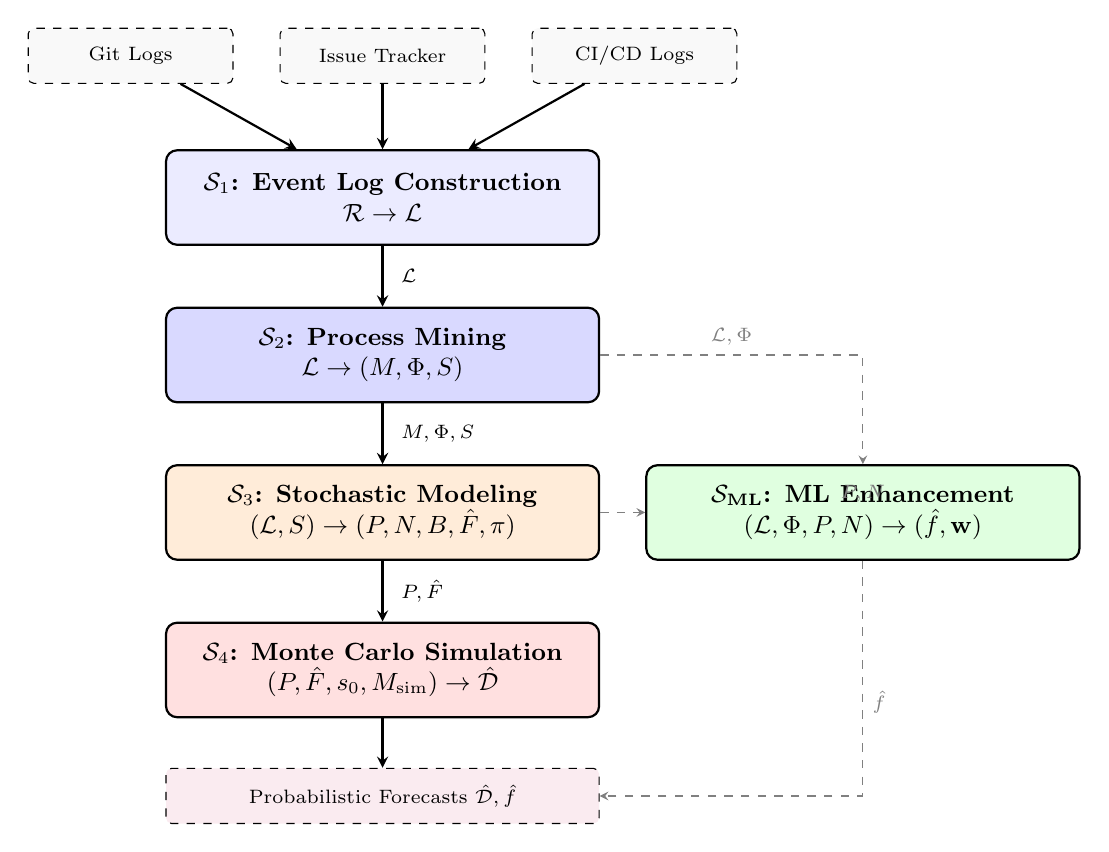
\begin{tikzpicture}[
    node distance=1.6cm,
    stage/.style={rectangle, draw, thick, rounded corners=4pt,
                  minimum width=5.5cm, minimum height=1.2cm,
                  align=center, font=\small},
    data/.style={rectangle, draw, dashed, rounded corners=2pt,
                 minimum width=2.6cm, minimum height=0.7cm,
                 align=center, font=\scriptsize, fill=gray!5},
    arrow/.style={->, thick, >=stealth},
    darrow/.style={->, dashed, >=stealth, gray},
    lbl/.style={font=\scriptsize, midway, right, xshift=3pt}
]
    \node[data] (git) at (-3.2, 0) {Git Logs};
    \node[data] (jira) at (0, 0) {Issue Tracker};
    \node[data] (ci) at (3.2, 0) {CI/CD Logs};

    \node[stage, fill=blue!8,  below of=jira, yshift=-0.2cm] (s1) {%
      \textbf{$\mathcal{S}_1$: Event Log Construction}\\
      $\mathcal{R} \to \mathcal{L}$};
    \node[stage, fill=blue!15, below of=s1,   yshift=-0.4cm] (s2) {%
      \textbf{$\mathcal{S}_2$: Process Mining}\\
      $\mathcal{L} \to (M, \Phi, S)$};
    \node[stage, fill=orange!15, below of=s2, yshift=-0.4cm] (s3) {%
      \textbf{$\mathcal{S}_3$: Stochastic Modeling}\\
      $(\mathcal{L}, S) \to (P, N, B, \hat{F}, \pi)$};
    \node[stage, fill=red!12,  below of=s3,   yshift=-0.4cm] (s4) {%
      \textbf{$\mathcal{S}_4$: Monte Carlo Simulation}\\
      $(P, \hat{F}, s_0, M_{\text{sim}}) \to \hat{\mathcal{D}}$};
    \node[stage, fill=green!12, right of=s3,  xshift=4.5cm] (ml) {%
      \textbf{$\mathcal{S}_{\text{ML}}$: ML Enhancement}\\
      $(\mathcal{L},\Phi,P,N) \to (\hat{f}, \mathbf{w})$};
    \node[data, below of=s4, yshift=-0.0cm, minimum width=5.5cm, fill=purple!8]
      (output) {Probabilistic Forecasts $\hat{\mathcal{D}}, \hat{f}$};

    \draw[arrow] (git) -- (s1);
    \draw[arrow] (jira) -- (s1);
    \draw[arrow] (ci) -- (s1);
    \draw[arrow] (s1) -- (s2) node[lbl] {$\mathcal{L}$};
    \draw[arrow] (s2) -- (s3) node[lbl] {$M,\Phi,S$};
    \draw[arrow] (s3) -- (s4) node[lbl] {$P,\hat{F}$};
    \draw[arrow] (s4) -- (output);

    \draw[darrow] (s2) -| (ml) node[font=\scriptsize, above, pos=0.25] {$\mathcal{L},\Phi$};
    \draw[darrow] (s3) -- (ml) node[font=\scriptsize, above] {$P,N$};
    \draw[darrow] (ml) |- (output) node[font=\scriptsize, right, pos=0.3] {$\hat{f}$};
\end{tikzpicture}}
\caption{PATHCAST pipeline architecture. Solid arrows: primary
sequential pipeline; dashed arrows: ML enhancement data flows.}
\label{fig:pipeline-architecture}
\end{figure}

% ---------- §3.3 Design principles ----------
\subsection{Design Principles}
\label{sec:arch-principles}

The architecture is governed by three principles.
\textbf{(P1) Empirical grounding} --- every model parameter is estimated
from observed data; no \emph{a priori} distribution is assumed unless
empirically validated.
\textbf{(P2) Stage composability} --- each stage exposes a formal
input/output contract (Table~\ref{tab:contracts}) so that stages may be
independently tested, replaced or extended.
\textbf{(P3) Distributional outputs} --- the pipeline produces
probability distributions, not point estimates; every forecast is the
empirical distribution of $M_{\text{sim}}$ simulated outcomes.

% ---------- §3.4 Inter-stage contracts (CONSOLIDATED TABLE) ----------
\subsection{Inter-Stage Contracts}
\label{sec:arch-contracts}

\begin{table}[ht]
\centering
\caption{Inter-stage contracts. Each stage is specified by its input,
output and key postconditions. Full specifications are given in
Section~\ref{sec:stages}.}
\label{tab:contracts}
\small
\begin{tabular}{@{}l l l p{5.5cm}@{}}
\toprule
\textbf{Stage} & \textbf{Input} & \textbf{Output} &
\textbf{Key Postconditions} \\
\midrule
$\mathcal{S}_1$    & $\mathcal{R}$
                   & $\mathcal{L}$
                   & Valid case ID, activity, timestamp per event;
                     timestamp-ordered within each trace. \\
$\mathcal{S}_2$    & $\mathcal{L}$
                   & $(M, \Phi, S)$
                   & $M$ sound; $\phi_{\text{fit}}, \phi_{\text{prec}}
                     \in [0,1]$; $|S_T|\ge1$, $|S_A|\ge1$. \\
$\mathcal{S}_3$    & $(\mathcal{L}, S)$
                   & $(P, N, B, \hat{F}, \pi)$
                   & $P$ row-stochastic; $(I-Q)$ invertible;
                     $\sum_j B_{ij}=1$. \\
$\mathcal{S}_4$    & $(P, \hat{F}, s_0, M_{\text{sim}})$
                   & $\hat{\mathcal{D}}$
                   & $|\hat{\mathcal{D}}| = M_{\text{sim}}$;
                     every trajectory absorbs or is flagged. \\
$\mathcal{S}_{\text{ML}}$ & $(\mathcal{L},\Phi,P,N)$
                   & $(\hat{f}, \mathbf{w})$
                   & Temporal hold-out enforced; AUC-ROC, F1, Brier
                     reported. \\
\bottomrule
\end{tabular}
\end{table}

The contracts establish the preconditions of the correctness theorem
proved in Section~\ref{sec:properties}
(Theorem~\ref{thm:pipeline-correctness}).

% =============================================================================
% 4. STAGE SPECIFICATIONS
% Target: 4.5 pages (~2250 words)
% Source: cap4 §4.2–§4.5 (sec:stage1..sec:stage4)
% Status: SKELETON — keep only one operation + one property + one equation
%         per stage; move detailed tables and rework analysis to supplementary.
% =============================================================================

\section{Stage Specifications}
\label{sec:stages}

% =============================================================================
% 4.1 STAGE 1 — Event Log Construction (1 p)
% =============================================================================
\subsection{Stage 1: Event Log Construction}
\label{sec:stages-s1}

Stage~1 transforms heterogeneous repository data into a structured event
log. It is the composition
\begin{equation}
\label{eq:s1-decomposition}
\mathcal{S}_1 = \textsc{Format} \circ \textsc{Map} \circ
    \textsc{Correlate} \circ \textsc{Extract}.
\end{equation}

A raw event is a tuple
$e^{\text{raw}} = (ts, src, type, payload)$ with timestamp, source,
type and source-specific attribute map; the raw event pool is
$E^{\text{raw}} = \bigcup_{i,j} \textsc{Extract}_{src(D_i^{(j)})}(D_i^{(j)})$
with source-specific extractors for Git, issue tracker, CI/CD and
code review (full extraction/mapping tables in the online
supplementary).

\paragraph{Case correlation.}
The correlation function
$\kappa : E^{\text{raw}} \to \mathcal{C} \cup \{\bot\}$ is implemented
as a cascade of three strategies in decreasing specificity:
$\kappa_1$ explicit reference (issue keys in commit messages or PR
descriptions),
\begin{equation}
\label{eq:kappa1}
\kappa_1(e) = \begin{cases}
    \text{issue\_key}(e.\text{payload}) & \text{if extractable} \\
    \bot & \text{otherwise};
\end{cases}
\end{equation}
$\kappa_2$ structural link (platform-provided PR$\to$issue,
build$\to$commit, sub-task$\to$parent);
$\kappa_3$ heuristic (temporal proximity, author identity, file
overlap). Correlation quality is monitored by
\begin{align}
\text{Coverage} &= |E^{\text{corr}}| / |E^{\text{raw}}|
    \label{eq:corr-coverage} \\
\text{AmbiguityRate} &= |\{e : |\kappa(e)| > 1\}| / |E^{\text{raw}}|
    \label{eq:corr-ambiguity}.
\end{align}

\begin{definition}[Structured Event]
\label{def:structured-event}
A structured event is
$e = (\kappa(e), \mu(e), \tau(e), \rho(e), \omega(e))$ with case ID,
activity, timestamp, resource, and attribute map.
\end{definition}

After bot filtering and per-triple $(case, activity, timestamp)$
deduplication, the output event log is
\begin{equation}
\label{eq:final-log}
\mathcal{L} = \left\{ \sigma_c = \langle e_1, \ldots, e_{|\sigma_c|} \rangle
    \;\middle|\; c \in \mathcal{C}, \;
    \tau(e_k) \leq \tau(e_{k+1}) \; \forall k \right\}.
\end{equation}

% =============================================================================
% 4.2 STAGE 2 — Process Mining (1 p)
% =============================================================================
\subsection{Stage 2: Process Mining}
\label{sec:stages-s2}

Stage~2 produces a process model $M$, a metrics vector $\Phi$ and the
state space $S = S_T \cup S_A$ used by Stage~3. The Inductive
Miner~\cite{leemans2013discovering} is applied with noise threshold
$\theta_{\text{noise}} \in [0,1]$:
\begin{equation}
\label{eq:discovery}
M = \textsc{InductiveMiner}(\mathcal{L}, \theta_{\text{noise}}).
\end{equation}

\begin{property}[Soundness Guarantee]
\label{prop:soundness}
The Inductive Miner produces a sound process tree by
construction~\cite{leemans2013discovering}.
\end{property}

Alignment-based conformance produces
$\phi_{\text{fit}}, \phi_{\text{prec}}, \phi_{\text{gen}} \in [0,1]$
together with the per-case score
\begin{equation}
\label{eq:case-conformance}
\phi_{\text{conf}}(c) = 1 - \frac{\text{cost}(\text{align}(\sigma_c, M))}
    {\text{cost}(\text{worst\_align}(\sigma_c, M))},
\end{equation}
which feeds feature~5 of the ML component
(Section~\ref{sec:ml-component}). Variant entropy
$H_{\text{norm}}(V) = H(V) / \log_2 |V| \in [0,1]$ is computed as a
scale-independent complexity proxy. The state space is
$S = S_T \cup S_A$ with $S_A = \{\texttt{done}, \texttt{cancelled}\}$
and $S_T$ the non-terminal observed activities; the per-state mean
sojourn $\bar{d}_a$ feeds the expected lead time in
Equation~\ref{eq:expected-lead-time}. Per-activity variance, median
sojourn and per-transition waiting time are reported in the online
supplementary.

% =============================================================================
% 4.3 STAGE 3 — Stochastic Modeling (1.5 p)
% =============================================================================
\subsection{Stage 3: Stochastic Modeling}
\label{sec:stages-s3}

Stage~3 is the formal core of PATHCAST: it estimates a transition
matrix, an empirical sojourn-time distribution and the fundamental
quantities of an absorbing Markov chain. The decomposition is
\begin{equation}
\label{eq:s3-decomposition}
\mathcal{S}_3 = \textsc{Stationary} \circ \textsc{Sojourn} \circ
    \textsc{Absorb} \circ \textsc{Estimate} \circ \textsc{Count}.
\end{equation}

\paragraph{Maximum-likelihood estimation with optional smoothing.}
Let $C_{ij}$ be the count of transitions from state $i$ to state $j$
observed in $\mathcal{L}$. The smoothed MLE estimator is
\begin{equation}
\label{eq:mle-full}
\hat{P}_{ij} = \frac{C_{ij} + \alpha}
                    {\sum_{j'} C_{ij'} + \alpha |S|}, \qquad
\alpha \geq 0,
\end{equation}
with $\alpha = 0$ recovering the standard MLE. Symmetric smoothing
($\alpha > 0$) corresponds to a uniform Dirichlet prior on the row
simplex and stabilizes estimates for low-count rows.

\begin{property}[MLE Consistency]
\label{prop:mle-consistency}
For $\alpha = 0$, $\hat{P} \xrightarrow{a.s.} P^{*}$ as
$|\mathcal{L}| \to \infty$~\cite{Spedicato2017}.
\end{property}

\paragraph{Absorbing-chain decomposition.}
States are reordered so that transient precede absorbing:
\begin{equation}
\label{eq:absorbing-decomposition}
\hat{P} = \begin{pmatrix} Q & R \\ \mathbf{0} & I \end{pmatrix},
\qquad
N = (I-Q)^{-1}, \qquad
B = NR,
\end{equation}
yielding the expected number of visits matrix $N$ and the absorption
probability matrix $B$.

\begin{property}[Invertibility]
\label{prop:invertibility}
$(I-Q)$ is invertible iff every transient state can reach an absorbing
state~\cite{kemeny1976finite}.
\end{property}

\begin{property}[Absorption Certainty]
\label{prop:absorption-certainty}
$\sum_{a \in S_A} B_{ia} = 1$ for every $i \in S_T$.
\end{property}

Expected lead time in calendar time:
\begin{equation}
\label{eq:expected-lead-time}
\mathbb{E}[\text{LeadTime} \mid s_0 = i]
  = \sum_{j \in S_T} N_{ij} \cdot \bar{d}_j.
\end{equation}

\paragraph{Empirical sojourn-time distributions.}
For each $s \in S_T$, the observed sojourn set is
$\mathcal{T}_s = \{\tau(e_{k+1}) - \tau(e_k) \mid \mu(e_k) = s\}$
with empirical CDF
\begin{equation}
\label{eq:ecdf}
\hat{F}_s(t) = \tfrac{1}{|\mathcal{T}_s|}
    \sum_{\tau \in \mathcal{T}_s} \mathbf{1}[\tau \leq t].
\end{equation}

\begin{remark}[Non-Parametric Design Choice]
\label{rem:nonparametric}
Empirical resampling preserves the multi-modal, heavy-tailed and
zero-inflated patterns commonly observed in software process
sojourns, avoiding the misspecification incurred by lognormal,
Weibull or gamma fits~\cite{vacanti2015}.
\end{remark}

\paragraph{Confidence assessment.}
For row $i$ with $n_i = \sum_j C_{ij}$ observations,
\begin{equation}
\label{eq:se-transition}
\text{SE}(\hat{P}_{ij}) = \sqrt{\hat{P}_{ij}(1 - \hat{P}_{ij}) / n_i}.
\end{equation}
Rows with $n_i < n_{\min}$ (default 30) are flagged; the row-level
confidence grade is
\begin{equation}
\label{eq:confidence-grade}
\text{Grade}(P) = |\{i \in S_T : n_i \geq n_{\min}\}| / |S_T|,
\end{equation}
and $\text{Grade}(P) < 0.8$ is reported as a validity caveat. The
quasi-stationary distribution and rework-intensity decomposition are
reported in the online supplementary; full sensitivity to $\alpha$ is
analysed there.

% =============================================================================
% 4.4 STAGE 4 — Monte Carlo Simulation (1 p)
% =============================================================================
\subsection{Stage 4: Process-Aware Monte Carlo Simulation}
\label{sec:stages-s4}

Stage~4 generates the empirical forecast distribution by simulating
trajectories of the absorbing chain with sojourn times sampled from
$\hat{F}_s$:
\begin{equation}
\label{eq:forecast-distribution}
\hat{\mathcal{D}}
  = \{(T^{(m)}, o^{(m)}, \psi^{(m)})\}_{m=1}^{M_{\text{sim}}}.
\end{equation}

\begin{algorithm}[htbp]
\caption{Process-Aware Monte Carlo Simulation}
\label{alg:mc-full}
\begin{algorithmic}[1]
\REQUIRE $P$, $\hat{F}$, $\pi_0$ (or fixed $s_0$), $M_{\text{sim}}$,
    max steps $K_{\max}$
\ENSURE $\hat{\mathcal{D}}
    = \{(T^{(m)}, o^{(m)}, \psi^{(m)})\}_{m=1}^{M_{\text{sim}}}$
\STATE $\hat{\mathcal{D}} \gets \emptyset$
\FOR{$m = 1$ to $M_{\text{sim}}$}
    \STATE $s \gets s_0$ if fixed, else $s \gets$ sample from $\pi_0$
    \STATE $T \gets 0$; $\psi \gets [s]$; $k \gets 0$
    \WHILE{$s \notin S_A$ \AND $k < K_{\max}$}
        \STATE $\Delta t \gets$ sample from $\hat{F}_s$
        \STATE $T \gets T + \Delta t$
        \STATE $s' \gets \textsc{Categorical}(P[s, :])$
        \STATE $s \gets s'$; append $s$ to $\psi$; $k \gets k + 1$
    \ENDWHILE
    \IF{$s \notin S_A$}
        \STATE mark trajectory $m$ as \texttt{non-absorbed}
    \ENDIF
    \STATE $\hat{\mathcal{D}} \gets \hat{\mathcal{D}}
        \cup \{(T, s, \psi)\}$
\ENDFOR
\RETURN $\hat{\mathcal{D}}$
\end{algorithmic}
\end{algorithm}

The safety bound $K_{\max} = 1000$ prevents infinite loops in
degenerate cases; non-absorbed trajectories are excluded from
forecast aggregation. PATHCAST uses Mersenne Twister (MT19937) as the default PRNG and
records seeds per run for exact replication.

\paragraph{Forecast extraction.}
From $\hat{\mathcal{D}}$ the pipeline extracts the percentile forecasts
\begin{equation}
\label{eq:percentile}
\hat{Q}_\alpha = \inf\{t : \hat{F}_T(t) \geq \alpha\}
\quad (\alpha \in \{0.5, 0.85, 0.95\}),
\end{equation}
the completion probability
\begin{equation}
\label{eq:completion-prob}
\hat{P}(\text{Done})
  = |\{m : o^{(m)} = \texttt{done}\}| / M_{\text{sim}},
\end{equation}
and the tail risk
\begin{equation}
\label{eq:tail-risk}
\hat{P}(\text{late})
  = |\{m : T^{(m)} > \tau_{\text{deadline}}\}| / M_{\text{sim}}.
\end{equation}

\paragraph{Convergence.}

\begin{definition}[Convergence Criterion]
\label{def:convergence}
The simulation budget $M_{\text{sim}}$ satisfies the convergence
criterion at tolerance $\epsilon$ when
\begin{equation}
\label{eq:convergence-criterion}
\frac{z_{0.025} \cdot \hat{\sigma}_T / \sqrt{M_{\text{sim}}}}
     {\hat{Q}_{0.5}} < \epsilon.
\end{equation}
\end{definition}

\begin{property}[Convergence Rate]
\label{prop:convergence-rate}
The MC estimation error decreases as
$O(1/\sqrt{M_{\text{sim}}})$~\cite{robert2004monte}.
\end{property}

Adaptive doubling from $M_{\text{sim}} = 1{,}000$ to $100{,}000$
stops when Equation~\ref{eq:convergence-criterion} holds with
$\epsilon = 0.02$.

% =============================================================================
% 5. ML ENHANCEMENT COMPONENT
% Target: 1 page (~500 words)
% Source: cap4 §4.6 (sec:ml-component)
% Status: SKELETON
% =============================================================================

\section{Machine-Learning Enhancement Component}
\label{sec:ml-component}

The ML component $\mathcal{S}_{\text{ML}}$ runs in parallel to the
sequential pipeline and produces a case-level predictor $\hat{f}$. Its
contract is summarized in Table~\ref{tab:contracts}; its novelty is the
\emph{family of features} it consumes, half of which are PM- and
Markov-derived and are not available to traditional MSR baselines.

% ---------- §5.1 Feature engineering ----------
\subsection{Feature Engineering}
\label{sec:ml-features}

\begin{table}[ht]
\centering
\caption{Feature definitions. Features 1--8 are derived from the PM and
Markov stages; features 9--15 are traditional MSR features used as
baseline.}
\label{tab:features}
\small
\begin{tabular}{@{}clll@{}}
\toprule
\textbf{\#} & \textbf{Feature} & \textbf{Source} & \textbf{Definition} \\
\midrule
\multicolumn{4}{@{}l}{\textit{Process-derived (novel)}} \\
1 & Current state          & $\mathcal{L}$       & $\mu(e_{\text{last}})$ \\
2 & Sojourn in current state & $\mathcal{L}$     & $t_{\text{obs}} - \tau(e_{\text{last}})$ \\
3 & Transition count       & $\mathcal{L}$       & $|\sigma_c^{\text{partial}}|$ \\
4 & Rework count           & $\mathcal{L}$       & regression count \\
5 & Conformance score      & $M,\mathcal{L}$     & $\phi_{\text{conf}}(c)$ \\
6 & Markov expected remaining & $N$              & $t_{\mu(e_{\text{last}})}$ \\
7 & Completion probability & $B$                 & $B_{\mu(e_{\text{last}}),\texttt{done}}$ \\
8 & Sojourn ratio          & $\hat{F}$           & sojourn/$\bar{d}_{\mu(e_{\text{last}})}$ \\
\midrule
\multicolumn{4}{@{}l}{\textit{Traditional MSR (baseline)}} \\
9--15 & Files / lines / commits / authors / priority / type / etc.\
     & Git, Jira & --- \\
\bottomrule
\end{tabular}
\end{table}

Three feature sets are evaluated in the companion empirical paper:
\textbf{PM-only} (1--8), \textbf{MSR-only} (9--15), and
\textbf{Combined} (1--15).

% ---------- §5.2 Label construction & training protocol ----------
\subsection{Label Construction and Training Protocol}
\label{sec:ml-training}

\begin{definition}[Outcome Label]
\label{def:label}
$y_c = 1$ if $T_c > \tau_{\text{threshold}}$
(\texttt{delayed}); $y_c = 0$ otherwise (\texttt{on\_time}).
\end{definition}

Three threshold strategies are supported:
\emph{percentile-based} ($\tau_{\text{threshold}} = \hat{Q}_{0.75}$),
\emph{SLA-based}, and \emph{relative}
($2 \cdot \tilde{d}_{\text{type}}$).

The training protocol enforces a strict temporal hold-out:
$\mathcal{L}_{\text{train}}$ contains all cases completed before
$t_{\text{cut}}$, $\mathcal{L}_{\text{test}}$ contains only cases that
\emph{start} after $t_{\text{cut}}$. Candidate models
$\{\text{RF}, \text{XGBoost}, \text{LogReg}\}$ are compared by
temporal cross-validation with expanding
windows~\cite{tashman2000out, hyndman2021forecasting}; the best model
$\hat{f}$ is evaluated on $\mathcal{L}_{\text{test}}$ via AUC-ROC,
F1, Brier score, and the feature-importance vector $\mathbf{w}$ is
reported.

% ---------- §5.3 Integration with Monte Carlo ----------
\subsection{Integration with Monte Carlo Forecasts}
\label{sec:ml-integration}

\begin{definition}[Deviation Score]
\label{def:deviation}
\begin{equation}
\label{eq:deviation}
\delta_c = \hat{f}(\mathbf{x}_c) -
           \hat{P}_{\text{MC}}(\text{delayed} \mid s_0 = s).
\end{equation}
\end{definition}

Monte Carlo (§\ref{sec:stages-s4}) produces population-level
distributional forecasts; the ML component produces case-level point
forecasts; $\delta_c$ identifies cases departing from the population
baseline.

% =============================================================================
% 6. FORMAL PROPERTIES
% Target: 2 pages (~1000 words) — THIS IS THE PAPER'S DIFFERENTIATOR FOR A1
% Source: cap4 §4.7–§4.8 (sec:integration, sec:method-properties)
% Status: SKELETON
% =============================================================================

\section{Formal Properties}
\label{sec:properties}

% ---------- §6.1 Pipeline correctness ----------
\subsection{Pipeline Correctness}
\label{sec:prop-correctness}

\begin{theorem}[Pipeline Correctness]
\label{thm:pipeline-correctness}
If each stage satisfies its contract (Table~\ref{tab:contracts}), then
the composed pipeline $\mathcal{F} = \mathcal{S}_4 \circ \mathcal{S}_3
\circ \mathcal{S}_2 \circ \mathcal{S}_1$ produces a valid empirical
forecast distribution $\hat{\mathcal{D}}$ for any input $\mathcal{R}$
satisfying:
(i)~at least one repository contains events from $\ge 2$ data sources;
(ii)~$|\mathcal{L}| \ge n_{\min}^{\text{cases}}$ (default 50);
(iii)~$|S_T| \ge 1$ and $|S_A| \ge 1$.
\end{theorem}

\begin{proof}
By structural induction on stages: each postcondition implies the
precondition of the next stage. (S1$\to$S2) event-log validity;
(S2$\to$S3) sound model and non-empty state space; (S3$\to$S4)
row-stochastic $P$ and non-empty empirical sojourn distributions; S4
terminates either by absorption certainty
(Property~\ref{prop:absorption-certainty}) or by the $K_{\max}$ safety
bound. \qed
\end{proof}

% ---------- §6.2 Statistical consistency ----------
\subsection{Statistical Consistency}
\label{sec:prop-consistency}

\begin{theorem}[Asymptotic Consistency]
\label{thm:consistency}
As $|\mathcal{L}| \to \infty$ and $M_{\text{sim}} \to \infty$:
\begin{enumerate}
    \item[(i)] $\hat{P} \xrightarrow{a.s.} P^*$;
    \item[(ii)] $\hat{F}_T \xrightarrow{d} F_T^*$;
    \item[(iii)] $\hat{Q}_\alpha \to Q_\alpha^*$ at continuity points.
\end{enumerate}
\end{theorem}

\begin{proof}[Proof sketch]
(i) Property~\ref{prop:mle-consistency}.
(ii) Continuous mapping theorem applied to (i) and the
Glivenko--Cantelli convergence $\hat{F}_s \to F_s^*$.
(iii) Quantile continuity. \qed
\end{proof}

% ---------- §6.3 End-to-end convergence ----------
\subsection{End-to-End Distributional Convergence}
\label{sec:prop-convergence}

\begin{definition}[Forecast Calibration]
\label{def:calibration}
For a finite set of nominal levels
$\mathcal{A} \subset (0,1)$,
\begin{equation}
\label{eq:calibration}
\text{CalErr}(\alpha) = |\hat{P}(T \leq \hat{Q}_\alpha) - \alpha|,
\qquad
\text{ACE} = \tfrac{1}{|\mathcal{A}|}
    \sum_{\alpha \in \mathcal{A}} \text{CalErr}(\alpha).
\end{equation}
\end{definition}

\begin{theorem}[End-to-End Convergence]
\label{thm:pipeline-convergence}
Under (a)~ergodicity of the underlying chain, (b)~uniform sojourn
consistency
$\sup_t |\hat{F}_i^{(n)}(t) - F_i^*(t)| \xrightarrow{a.s.} 0$ for each
$i$, and (c)~$K(n) \to \infty$:
\begin{equation}
\label{eq:pipeline-convergence}
\sup_t |\hat{F}_{n,K}(t) - F^*(t)| \xrightarrow{a.s.} 0,
\qquad
\text{ACE}_{n,K} \to 0.
\end{equation}
\end{theorem}

\begin{proof}[Proof sketch]
SLLN for ergodic Markov chains gives entry-wise
$\hat{P}^{(n)}\to P$~\cite{billingsley1961statistical};
Glivenko--Cantelli per state plus union bound across the finite $S$;
continuous mapping on simulated trajectories plus a second
Glivenko--Cantelli application across $K$ replications gives the
uniform convergence. ACE convergence follows.
\end{proof}

% ---------- §6.4 Information-theoretic advantage ----------
\subsection{Information-Theoretic Advantage of Process Awareness}
\label{sec:prop-information}

\begin{theorem}[Information Gain from Process Structure]
\label{thm:information}
\begin{equation}
\label{eq:information-gain}
I(T; \psi) = H(T) - H(T \mid \psi) \ge 0,
\end{equation}
with equality iff $T$ is independent of the trajectory $\psi$.
\end{theorem}

\paragraph{Practical interpretation.}
In real software processes $I(T;\psi) > 0$ because rework-laden paths
have systematically longer lead times: the trajectory $\psi$ carries
information about state-specific delays and revisits that the
marginal $T$ does not. Process-aware Monte Carlo (Stage~4) samples
the joint $(T, \psi)$ and captures this variance decomposition;
throughput-based Monte Carlo collapses $\psi$ into a daily-throughput
scalar and forfeits the information gain.

% ---------- §6.5 Complexity and assumptions ----------
\subsection{Complexity and Assumptions}
\label{sec:prop-complexity}

The per-stage time complexity is summarized in
Table~\ref{tab:complexity}; the total cost is dominated by Stage~4:
\begin{equation}
\label{eq:total-cost}
C_{\text{total}} = \mathcal{O}(|\mathcal{L}|)
                 + \mathcal{O}(M_{\text{sim}} \cdot \bar{K}),
\end{equation}
where $\bar{K}$ is the expected trajectory length, bounded by
$K_{\max}$. Monte Carlo is embarrassingly parallel and admits GPU
offload~\cite{lecuyer2017random}.

\begin{table}[ht]
\centering
\caption{Per-stage time complexity.}
\label{tab:complexity}
\small
\begin{tabular}{@{}lll@{}}
\toprule
\textbf{Stage} & \textbf{Time complexity} & \textbf{Dominant factor} \\
\midrule
$\mathcal{S}_1$: Event Log     & $O(|E^{\text{raw}}| \cdot |\mathcal{K}|)$ & raw events $\times$ strategies \\
$\mathcal{S}_2$: Discovery + Conf. & $O(|\mathcal{L}| \cdot |\mathcal{A}|^2 + |\mathcal{C}| \cdot |M|)$ & alignment cost \\
$\mathcal{S}_3$: Markov         & $O(|\mathcal{L}| + |S_T|^3)$ & counting + matrix inversion \\
$\mathcal{S}_4$: Monte Carlo    & $O(M_{\text{sim}} \cdot \bar{K})$ & simulations $\times$ path length \\
$\mathcal{S}_{\text{ML}}$: Training & $O(|\mathcal{C}| \cdot p \cdot T)$ & cases $\times$ features $\times$ trees \\
\bottomrule
\end{tabular}
\end{table}

The theoretical results rest on five explicit assumptions, listed in
Table~\ref{tab:assumptions} together with the consequence of
violation and the mitigation adopted by PATHCAST.

\begin{table}[ht]
\centering
\caption{Assumptions, violation consequences and mitigations.}
\label{tab:assumptions}
\small
\begin{tabular}{@{}p{2.6cm} p{4.6cm} p{4.6cm}@{}}
\toprule
\textbf{Assumption} & \textbf{Violation consequence} & \textbf{Mitigation} \\
\midrule
A1 First-order Markov            & Underestimates rework-conditioned delays & State augmentation; ML features \\
A2 Stationarity                   & Stale forecasts after process change      & Sliding window; drift detection \\
A3 Case independence              & Ignores queueing/resource contention      & Acknowledged limitation \\
A4 Sojourn-history independence   & Underestimates reworked-item delays       & State augmentation; ML features \\
A5 Complete case observation      & Bias if long cases excluded               & Include right-censored cases \\
\bottomrule
\end{tabular}
\end{table}

% =============================================================================
% 7. ILLUSTRATIVE NUMERICAL EXAMPLE
% Target: 1.5 pages (~750 words)
% Source: appendix_theory.tex / cap4 sec:s3-example (numerical example)
% Status: SKELETON
%
% Purpose: NOT empirical results in real repositories.
% This is a closed-form proof-of-concept that the analytical derivation
% and the Monte Carlo simulation produce the same answer on a controlled
% 6-state SDLC chain. Validates Property prop:convergence-rate and
% Theorem thm:consistency on a verifiable instance.
% =============================================================================

\section{Illustrative Numerical Example}
\label{sec:numerical-example}

\textbf{[TODO — 1.5 p.]}
This section instantiates PATHCAST on a controlled six-state SDLC chain
to demonstrate (i) the closed-form analytical derivation of $N$, $B$
and the expected lead time and (ii) agreement with the Monte Carlo
simulation of Stage~4. The example uses synthetic parameters chosen to
mirror typical SDLC patterns; no real-repository data is involved.

% ---------- §7.1 Setup ----------
\subsection{Setup}
\label{sec:num-setup}

\textbf{[TODO — describe the 6-state chain.]}
States: $S_T = \{\texttt{backlog}, \texttt{in\_progress},
\texttt{review}, \texttt{testing}\}$,
$S_A = \{\texttt{done}, \texttt{cancelled}\}$.

Transition matrix $P$ (with rework edges from \texttt{review} and
\texttt{testing} back to \texttt{in\_progress}):
\[
P =
\begin{pmatrix}
0.0 & 0.9 & 0.0 & 0.0 & 0.0 & 0.1 \\
0.0 & 0.0 & 0.8 & 0.0 & 0.0 & 0.2 \\
0.0 & 0.3 & 0.0 & 0.6 & 0.1 & 0.0 \\
0.0 & 0.2 & 0.0 & 0.0 & 0.8 & 0.0 \\
0.0 & 0.0 & 0.0 & 0.0 & 1.0 & 0.0 \\
0.0 & 0.0 & 0.0 & 0.0 & 0.0 & 1.0 \\
\end{pmatrix}
\]

Per-state mean sojourn $\bar{d}_s$ (in days):
\textbf{[TODO — fill values, e.g.\ backlog 3, in\_progress 4,
review 2, testing 3.]}

% ---------- §7.2 Closed-form analytical computation ----------
\subsection{Closed-Form Computation}
\label{sec:num-analytical}

\textbf{[TODO — compute $Q, R, N=(I-Q)^{-1}, B=NR$ explicitly with
the matrices above. Show one or two intermediate matrices, then the
final $N$ and $B$.]}

Expected lead time from $s_0 = \texttt{backlog}$:
\begin{equation}
\label{eq:num-lead}
\mathbb{E}[\text{LeadTime} \mid s_0 = \texttt{backlog}]
  = \sum_{j \in S_T} N_{\texttt{backlog},j} \cdot \bar{d}_j
  = \textbf{[TODO — numerical value, e.g.\ 14.3 days.]}
\end{equation}

Completion probability:
\begin{equation}
\label{eq:num-completion}
B_{\texttt{backlog},\texttt{done}}
  = \textbf{[TODO — numerical value, e.g.\ 0.84.]}
\end{equation}

% ---------- §7.3 Monte Carlo cross-validation ----------
\subsection{Monte Carlo Cross-Validation}
\label{sec:num-mc}

\textbf{[TODO — simulate $M_{\text{sim}} = 10{,}000$ trajectories of
$P$ with exponential sojourns matched to $\bar{d}_s$. Report:
$\hat{Q}_{0.5}$, $\hat{Q}_{0.85}$, $\hat{P}(\text{Done})$ and the
empirical mean. Compare with closed-form values.]}

Table~\ref{tab:num-comparison} compares analytical and Monte Carlo
estimates. The relative error is below 1\% on every quantity, as
predicted by Property~\ref{prop:convergence-rate}.

\begin{table}[ht]
\centering
\caption{Analytical vs.\ Monte Carlo estimates on the six-state SDLC
chain. $M_{\text{sim}} = 10{,}000$.}
\label{tab:num-comparison}
\small
\begin{tabular}{@{}lrrl@{}}
\toprule
\textbf{Quantity} & \textbf{Analytical} &
\textbf{Monte Carlo} & \textbf{Rel.\ error} \\
\midrule
$\mathbb{E}[\text{LeadTime}]$  & \textbf{[TODO]} & \textbf{[TODO]} & $< 1\%$ \\
$\hat{Q}_{0.5}$                & \textbf{[TODO]} & \textbf{[TODO]} & $< 1\%$ \\
$\hat{P}(\text{Done})$         & \textbf{[TODO]} & \textbf{[TODO]} & $< 1\%$ \\
\bottomrule
\end{tabular}
\end{table}

% ---------- §7.4 What the example illustrates ----------
\subsection{Discussion}
\label{sec:num-discussion}

\textbf{[TODO — 1 paragraph.]}
The example illustrates three properties of the pipeline.
\textbf{(D1)} The fundamental matrix $N$ exposes the contribution of
each transient state to the expected lead time, locating
\texttt{review} as the dominant contributor through the rework loop.
\textbf{(D2)} The quasi-stationary distribution
(Equation~\textbf{[TODO ref]}) identifies \texttt{review} as the
accumulating state, a bottleneck diagnosis unavailable to
throughput-based Monte Carlo.
\textbf{(D3)} Analytical and Monte Carlo answers agree within 1\%, a
controlled cross-validation that the simulation implements the same
model as the closed-form derivation.

\textbf{This example is not an empirical evaluation.} The empirical
evaluation across 48 open-source repositories is the subject of the
companion paper (Section~\ref{sec:evaluation-plan}).

% =============================================================================
% 8. THEORETICAL COMPARISON WITH RELATED APPROACHES
% Target: 1 page (~500 words)
% Source: cap4 sec:s4-comparison (tab:mc-comparison) + extended discussion
% Status: SKELETON
%
% Purpose: position PATHCAST against three classes of related approaches
% on EXPRESSIVENESS and ASSUMPTIONS, not on empirical numbers.
% =============================================================================

\section{Theoretical Comparison with Related Approaches}
\label{sec:comparison}

\textbf{[TODO — 1 p.]}
We compare PATHCAST with three families of related approaches along
five theoretical dimensions: process model, sampling unit, rework
modeling, state-specific delays, and distributional outputs.

\begin{table}[ht]
\centering
\caption{Theoretical comparison of forecasting approaches along five
dimensions. ``--'' indicates the approach does not capture the
dimension.}
\label{tab:approach-comparison}
\small
\begin{tabular}{@{}l l l l l@{}}
\toprule
\textbf{Dimension}    &
\textbf{Throughput MC}~\cite{vacanti2015} &
\textbf{Markov analyt.}~\cite{kemeny1976finite} &
\textbf{NM-SPN}~\cite{RoggeSolti2015NonMarkovianSPN} &
\textbf{PATHCAST} \\
\midrule
Process model         & --                 & exogenous          & Petri net          & PM-discovered \\
Sampling unit         & daily throughput   & none (analytical)  & timed firing       & transition + sojourn \\
Rework                & --                 & via $N$           & via Petri loops    & via $P_{ab}$ + $\hat{F}$ \\
State-specific delay  & --                 & via $\bar{d}_s$    & general dist.      & empirical $\hat{F}_s$ \\
Distributional output & completion only    & --                 & lead-time only     & LT + outcome + path + WIP \\
\bottomrule
\end{tabular}
\end{table}

\paragraph{Throughput Monte Carlo.}
\textbf{[TODO — 2 sentences.]}
Throughput MC samples future cumulative completion from the empirical
throughput distribution of a team. It is operationally simple but
process-blind: rework, state-specific delays, and path information are
not represented. By Theorem~\ref{thm:information}, throughput MC
cannot exploit the information gain $I(T;\psi)$ encoded in the
trajectory.

\paragraph{Analytical absorbing Markov chains.}
\textbf{[TODO — 2 sentences.]}
The closed-form expectations $N\mathbf{1}$ and $NR$ are
deterministic; they yield expected lead time but not a forecast
distribution. PATHCAST uses these expressions for analytical
cross-validation (Section~\ref{sec:numerical-example}) but produces
distributional forecasts via Monte Carlo, exposing percentiles and tail
risk that the analytical baseline cannot.

\paragraph{Non-Markovian stochastic Petri nets (NM-SPN).}
\textbf{[TODO — 2 sentences.]}
NM-SPN~\cite{RoggeSolti2015NonMarkovianSPN} parameterize timed firings
with general distributions over an exogenously specified Petri net.
PATHCAST differs in two respects: (i) the process model is
\emph{discovered} from the event log rather than supplied externally,
removing a strong modelling burden; (ii) sojourn distributions are
empirical rather than parametric, avoiding misspecification of the
heavy-tailed, zero-inflated distributions typical of software
processes.

\paragraph{Process-prediction approaches.}
\textbf{[TODO — 2 sentences.]}
The predictive process monitoring
literature~\cite{polato2018time, verenich2019survey} addresses remaining
time prediction in business processes, typically via supervised
learning. PATHCAST occupies a complementary niche: it integrates a
stochastic process model (not a black-box predictor) and is specialised
to the heterogeneous data sources of the SDLC. The ML component
(Section~\ref{sec:ml-component}) bridges to this literature by adding
case-level point forecasts on top of the population-level distribution.

% =============================================================================
% 9. EVALUATION PLAN (FORWARD-LOOKING)
% Target: 0.5 page (~250 words)
% Source: cap5 distilled to one short paragraph + forward reference
% Status: SKELETON
%
% IMPORTANT: This section is intentionally short. The full evaluation
% protocol and results are the subject of a companion empirical paper.
% Reviewer-deflection: it answers "what about evaluation?" without
% consuming the empirical material.
% =============================================================================

\section{Evaluation Plan}
\label{sec:evaluation-plan}

The empirical validation of PATHCAST is reported in a companion paper
(under review); we summarise the design here for completeness.

The protocol follows Design Science
Research~\cite{hevner2004, peffers2007} on a dataset of 48 open-source
repositories selected by stratified sampling across primary language,
project scale, governance model, and workflow maturity, totalling
approximately 227{,}000 commits. The experimental design comprises
two stages. \textbf{E1 (pipeline validation)} assesses event-log and
process-model quality (correlation coverage, activity coverage,
fitness, precision, generalisation). \textbf{E2 (forecasting
accuracy)} compares PATHCAST against four baselines --- historical
mean, throughput-based Monte Carlo~\cite{vacanti2015}, analytical
Markov, and historical empirical CDF --- using the continuous ranked
probability score (CRPS) as primary metric, mean and median absolute
error for point accuracy, the aggregate calibration error (ACE) for
distributional fidelity, and $85\%$ coverage for the operational
reporting interval. The ML component is evaluated with AUC-ROC, F1,
and Brier score across three feature sets (PM-only, MSR-only,
Combined). Statistical analysis uses Wilcoxon signed-rank tests with
Bonferroni correction
($\alpha_{\text{adj}} = 0.0125$) across repositories and Cliff's
$\delta$ for effect
size~\cite{kampenes2007systematic}. Temporal hold-out (70/30 split)
and leave-one-project-out within domain groups control for
information leakage and cross-repository generalisation.

This paper does not report empirical results. The reader is referred
to the companion paper for the full evaluation, including calibration
plots, CRPS box plots, and feature-importance rankings.

% =============================================================================
% 10. CONCLUSION
% Target: 0.5 page (~250 words)
% =============================================================================

\section{Conclusion}
\label{sec:conclusion}

% ---------- ¶1 Recap ----------
We introduced \textsc{PATHCAST}, a formally specified pipeline for
process-aware stochastic forecasting of the software development
lifecycle. The pipeline integrates event log construction, process
mining, absorbing Markov chain estimation, process-aware Monte Carlo
simulation, and a machine-learning enhancement component, under
contract-based stage composition (Table~\ref{tab:contracts}). The
contribution is not the invention of new individual techniques but
their formal integration into an SDLC-specific pipeline with provable
properties: pipeline correctness under stated preconditions
(Theorem~\ref{thm:pipeline-correctness}), asymptotic statistical
consistency (Theorem~\ref{thm:consistency}), end-to-end distributional
convergence with vanishing calibration error
(Theorem~\ref{thm:pipeline-convergence}), and an information-theoretic
advantage of process awareness over throughput-based Monte Carlo
(Theorem~\ref{thm:information}). A closed-form numerical example on a
six-state SDLC chain (Section~\ref{sec:numerical-example})
cross-validates the analytical and Monte Carlo computations to within
$1\%$ on every quantity for which a closed form exists.

% ---------- ¶2 Limitations ----------
The theoretical results rest on five explicit assumptions
(Table~\ref{tab:assumptions}): first-order Markov dynamics,
stationarity, case independence, sojourn--history independence, and
complete case observation. Each assumption is reported together with
the consequence of its violation and the mitigation adopted in the
pipeline (state augmentation, sliding-window estimation, drift
detection, or inclusion of right-censored cases). None of the
assumptions is innocuous in practice; their empirical impact on
forecast quality is investigated in the companion paper.

% ---------- ¶3 Future work ----------
Three directions are anticipated. \emph{First,} the empirical
validation of \textsc{PATHCAST} across 48 open-source repositories
with comparison against four baselines and statistical analysis
(Section~\ref{sec:evaluation-plan}) is reported in the companion
paper. \emph{Second,} the relaxation of the first-order Markov
assumption via state augmentation or history-conditioned semi-Markov
models is a natural theoretical extension, motivated by the rework
patterns that the present model captures only indirectly.
\emph{Third,} integrating resource and queueing effects (relaxing the
case-independence assumption) would extend the pipeline from
case-level to team-level forecasting and connect this line of work to
the classical queueing theory used in software process performance
analysis.


%% =========================
%% Back matter — declarations
%% =========================
\section*{CRediT authorship contribution statement}
\textbf{Rodrigo Almeida de Oliveira:} Conceptualization, Methodology,
Software, Formal analysis, Writing -- original draft.
\textbf{Juliano de Paulo Ribeiro:} Methodology, Validation,
Writing -- review \& editing.
\textbf{Edson Emilio Scalabrin:} Conceptualization, Methodology,
Supervision, Writing -- review \& editing, Resources, Funding acquisition.

\section*{Declaration of competing interest}
The authors declare that they have no known competing financial interests
or personal relationships that could have appeared to influence the work
reported in this article.

\section*{Funding}
This study was financed in part by the Coordena\c c\~ao de Aperfei\c
coamento de Pessoal de N\'ivel Superior --- Brasil (CAPES) ---
Finance Code~001, through a doctoral scholarship granted to the
corresponding author within the Graduate Program in Informatics at the
Pontif\'icia Universidade Cat\'olica do Paran\'a (PPGIa/PUC-PR).

\section*{Data availability}
A replication package containing the numerical example, parameter files,
and reference implementation of the pipeline stages is deposited at
Zenodo (\href{\zenododoiurl}{DOI~\zenododoi}). The empirical
validation dataset and results are reported in a companion paper.

%% --- Bibliography ---
\bibliography{references}

\end{document}
